\chapter{E-commerce background} \label{chap:ecommerce}

\section*{}

% Neste capítulo é descrito o estado da arte e são
%apresentados trabalhos relacionados para mostrar o que existe no
%mesmo domínio e quais os problemas em aberto.
%Deve deixar claro que existe uma oportunidade de desenvolvimento que
%cobre alguma falha concreta .

%O capítulo deve também efetuar uma revisão tecnológica às principais
%ferramentas utilizáveis no âmbito do projeto, justificando futuras
%escolhas.

\section{Introduction}

Customer Behavior Model Graph (CBMG) <---

\section{Customer life cycle}

\begin{figure}[h]
  \begin{center}
    \leavevmode
    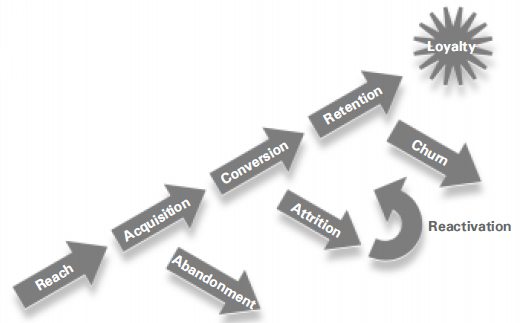
\includegraphics[width=0.86\textwidth]{lifecycle}
    \caption{Customer lifecycle \cite{Sterne2000}}
    \label{fig:lifecycle}
  \end{center}
\end{figure}

Reach -> Acquisition/Abandonment -> Conversion/Attrition -> Retention / Churn -> Loyalty

\section{E-commerce metrics}

\cite{Sterne2000}

\section{Influencing user behaviour}

-> influenciar behaviour em vez de recom

\subsection{Recommendation engines}

\cite{Adomavicius2005}

\section{Summary}

No final do capítulo deverá ser apresentado um resumo com as 
principais conclusões que se podem tirar. 
